%Chapter 6
\chapter{Funciones productivas}

Muchas de las funciones de Python que hemos utilizado, como las funciones matemáticas, producen valores de retorno. Pero las funciones que hemos escrito son todas nulas: tienen un efecto, como imprimir un valor o mover una tortuga, pero no tienen un valor de retorno. En este capítulo aprenderás a escribir funciones productivas.

\section{Valores de retorno}

Llamar a la función genera un valor de retorno, que normalmente asignamos a una variable o usamos como parte de una expresión.

\begin{lstlisting}[language=Python]
e = math.exp(1.0)
height = radius * math.sin(radians)
\end{lstlisting}

Las funciones que hemos escrito hasta ahora son nulas. Hablando informalmente, no tienen valor de retorno; más precisamente, su valor de retorno es \texttt{None}.

En este capítulo, vamos (finalmente) a escribir funciones productivas. El primer ejemplo es \texttt{area}, que devuelve el área de un círculo con el radio dado:

\begin{lstlisting}[language=Python]
def area(radius):
    a = math.pi * radius**2
    return a
\end{lstlisting}

Hemos visto la sentencia \texttt{return} antes, pero en una función productiva la sentencia \texttt{return} incluye una expresión. Esta sentencia significa: "Retorna inmediatamente de esta función y usa la siguiente expresión como valor de retorno". La expresión puede ser arbitrariamente complicada, así que podríamos haber escrito esta función de manera más concisa:

\begin{lstlisting}[language=Python]
def area(radius):
    return math.pi * radius**2
\end{lstlisting}

Por otro lado, las \textbf{variables temporales} como \texttt{a} pueden facilitar la depuración.

A veces es útil tener múltiples sentencias \texttt{return}, una en cada rama de un condicional:

\begin{lstlisting}[language=Python]
def absolute_value(x):
    if x < 0:
        return -x
    else:
        return x
\end{lstlisting}

Como estas sentencias \texttt{return} están en un condicional alternativo, solo una se ejecuta.

Tan pronto como se ejecuta una sentencia \texttt{return}, la función termina sin ejecutar ninguna sentencia posterior. El código que aparece después de una sentencia \texttt{return}, o cualquier otro lugar al que el flujo de ejecución nunca pueda llegar, se llama \textbf{código muerto}.

En una función productiva, es una buena idea asegurarse de que cada posible camino a través del programa llegue a una sentencia \texttt{return}. Por ejemplo:

\begin{lstlisting}[language=Python]
def absolute_value(x):
    if x < 0:
        return -x
    if x > 0:
        return x
\end{lstlisting}

Esta función es incorrecta porque si \texttt{x} es 0, ninguna condición es verdadera y la función termina sin llegar a una sentencia \texttt{return}. Si el flujo de ejecución llega al final de una función, el valor de retorno es \texttt{None}, que no es el valor absoluto de 0.

\begin{lstlisting}[language=Python]
>>> print(absolute_value(0))
None
\end{lstlisting}

Por cierto, Python proporciona una función incorporada llamada \texttt{abs} que calcula valores absolutos.

Como ejercicio, escribe una función \texttt{compare} que tome dos valores, \texttt{x} e \texttt{y}, y devuelva 1 si \texttt{x > y}, 0 si \texttt{x == y}, y -1 si \texttt{x < y}.

\section{Desarrollo incremental}

A medida que escribes funciones más grandes, podrías encontrarte pasando más tiempo depurando.

Para manejar programas cada vez más complejos, es posible que desees probar un proceso llamado \textbf{desarrollo incremental}. El objetivo del desarrollo incremental es evitar largas sesiones de depuración agregando y probando solo una pequeña cantidad de código a la vez.

Como ejemplo, supongamos que deseas encontrar la distancia entre dos puntos, dados por las coordenadas $(x_1, y_1)$ y $(x_2, y_2)$. Por el teorema de Pitágoras, la distancia es:

\[
\text{distancia} = \sqrt{(x_2 - x_1)^2 + (y_2 - y_1)^2}
\]

El primer paso es considerar cómo debería verse una función \texttt{distance} en Python. En otras palabras, ¿cuáles son las entradas (parámetros) y cuál es la salida (valor de retorno)?

En este caso, las entradas son dos puntos, que puedes representar usando cuatro números. El valor de retorno es la distancia representada por un valor de punto flotante.

Inmediatamente puedes escribir un esquema de la función:

\begin{lstlisting}[language=Python]
def distance(x1, y1, x2, y2):
    return 0.0
\end{lstlisting}

Obviamente, esta versión no calcula distancias; siempre devuelve cero. Pero es sintácticamente correcta y se ejecuta, lo que significa que puedes probarla antes de hacerla más complicada.

Para probar la nueva función, llámala con argumentos de muestra:

\begin{lstlisting}[language=Python]
>>> distance(1, 2, 4, 6)
0.0
\end{lstlisting}

Elegí estos valores para que la distancia horizontal sea 3 y la distancia vertical sea 4; de esa manera, el resultado es 5, la hipotenusa de un triángulo rectángulo 3-4-5. Al probar una función, es útil conocer la respuesta correcta.

En este punto hemos confirmado que la función es sintácticamente correcta y podemos comenzar a agregar código al cuerpo. Un siguiente paso razonable es encontrar las diferencias $x_2 - x_1$ y $y_2 - y_1$. La siguiente versión almacena esos valores en variables temporales y los imprime.

\begin{lstlisting}[language=Python]
def distance(x1, y1, x2, y2):
    dx = x2 - x1
    dy = y2 - y1
    print('dx is', dx)
    print('dy is', dy)
    return 0.0
\end{lstlisting}

Si la función está funcionando, debería mostrar \texttt{dx is 3} y \texttt{dy is 4}. Si es así, sabemos que la función está recibiendo los argumentos correctos y realizando el primer cálculo correctamente. Si no, solo hay unas pocas líneas para revisar.

Luego calculamos la suma de los cuadrados de \texttt{dx} y \texttt{dy}:

\begin{lstlisting}[language=Python]
def distance(x1, y1, x2, y2):
    dx = x2 - x1
    dy = y2 - y1
    dsquared = dx**2 + dy**2
    print('dsquared is: ', dsquared)
    return 0.0
\end{lstlisting}

Nuevamente, ejecutarías el programa en esta etapa y verificarías la salida (que debería ser 25). Finalmente, puedes usar \texttt{math.sqrt} para calcular y devolver el resultado:

\begin{lstlisting}[language=Python]
def distance(x1, y1, x2, y2):
    dx = x2 - x1
    dy = y2 - y1
    dsquared = dx**2 + dy**2
    result = math.sqrt(dsquared)
    return result
\end{lstlisting}

Si eso funciona correctamente, has terminado. De lo contrario, podrías imprimir el valor de \texttt{result} antes de la sentencia \texttt{return}.

La versión final de la función no muestra nada cuando se ejecuta; solo devuelve un valor. Las sentencias \texttt{print} que escribimos son útiles para depurar, pero una vez que la función funciona, deberías eliminarlas. Ese tipo de código se llama \textbf{andamiaje} porque es útil para construir el programa pero no es parte del producto final.

Cuando comienzas, solo deberías agregar una o dos líneas de código a la vez. A medida que ganes más experiencia, podrías encontrarte escribiendo y depurando fragmentos más grandes. De cualquier manera, el desarrollo incremental puede ahorrarte mucho tiempo de depuración.

Los aspectos clave del proceso son:

\begin{enumerate}
    \item Comienza con un programa que funcione y haz pequeños cambios incrementales. En cualquier punto, si hay un error, deberías tener una buena idea de dónde está.
    \item Usa variables para contener valores intermedios para que puedas mostrarlos y verificarlos.
    \item Una vez que el programa funcione, podrías eliminar parte del andamiaje o consolidar múltiples sentencias en expresiones compuestas, pero solo si no dificulta la lectura del programa.
\end{enumerate}

Como ejercicio, usa el desarrollo incremental para escribir una función llamada \texttt{hypotenuse} que devuelva la longitud de la hipotenusa de un triángulo rectángulo dados los largos de los otros dos lados como argumentos. Registra cada etapa del proceso de desarrollo a medida que avanzas.

\section{Composición}

Como ya deberías esperar, puedes llamar a una función desde dentro de otra. Como ejemplo, escribiremos una función que tome dos puntos, el centro del círculo y un punto en el perímetro, y calcule el área del círculo.

Supongamos que el punto central está almacenado en las variables \texttt{xc} e \texttt{yc}, y el punto del perímetro está en \texttt{xp} e \texttt{yp}. El primer paso es encontrar el radio del círculo, que es la distancia entre los dos puntos. Acabamos de escribir una función, \texttt{distance}, que hace eso:

\begin{lstlisting}[language=Python]
radius = distance(xc, yc, xp, yp)
\end{lstlisting}

El siguiente paso es encontrar el área de un círculo con ese radio; también acabamos de escribir eso:

\begin{lstlisting}[language=Python]
result = area(radius)
\end{lstlisting}

Encapsulando estos pasos en una función, obtenemos:

\begin{lstlisting}[language=Python]
def circle_area(xc, yc, xp, yp):
    radius = distance(xc, yc, xp, yp)
    result = area(radius)
    return result
\end{lstlisting}

Las variables temporales \texttt{radius} y \texttt{result} son útiles para el desarrollo y la depuración, pero una vez que el programa funciona, podemos hacerlo más conciso componiendo las llamadas a funciones:

\begin{lstlisting}[language=Python]
def circle_area(xc, yc, xp, yp):
    return area(distance(xc, yc, xp, yp))
\end{lstlisting}

\section{Funciones booleanas}

Las funciones pueden devolver booleanos, lo que a menudo es conveniente para ocultar pruebas complicadas dentro de funciones. Por ejemplo:

\begin{lstlisting}[language=Python]
def is_divisible(x, y):
    if x % y == 0:
        return True
    else:
        return False
\end{lstlisting}

Es común dar a las funciones booleanas nombres que suenen como preguntas de sí/no; \texttt{is\_divisible} devuelve \texttt{True} o \texttt{False} para indicar si \texttt{x} es divisible por \texttt{y}.

Aquí hay un ejemplo:

\begin{lstlisting}[language=Python]
>>> is_divisible(6, 4)
False
>>> is_divisible(6, 3)
True
\end{lstlisting}

El resultado del operador \texttt{==} es un booleano, por lo que podemos escribir la función de manera más concisa devolviéndolo directamente:

\begin{lstlisting}[language=Python]
def is_divisible(x, y):
    return x % y == 0
\end{lstlisting}

Las funciones booleanas se usan a menudo en sentencias condicionales:

\begin{lstlisting}[language=Python]
if is_divisible(x, y):
    print('x is divisible by y')
\end{lstlisting}

Podría ser tentador escribir algo como:

\begin{lstlisting}[language=Python]
if is_divisible(x, y) == True:
    print('x is divisible by y')
\end{lstlisting}

Pero la comparación adicional es innecesaria. Como ejercicio, escribe una función \texttt{is\_between(x, y, z)} que devuelva \texttt{True} si $x \leq y \leq z$ o \texttt{False} en caso contrario.

\section{Más recursión}

Hemos cubierto solo un pequeño subconjunto de Python, pero te podría interesar saber que este subconjunto es un lenguaje de programación \textit{completo}, lo que significa que cualquier cosa que se pueda calcular se puede expresar en este lenguaje. Cualquier programa escrito podría reescribirse usando solo las características del lenguaje que has aprendido hasta ahora (en realidad, necesitarías algunos comandos para controlar dispositivos como el mouse, discos, etc., pero eso es todo).

Probar esa afirmación es un ejercicio no trivial realizado por primera vez por Alan Turing, uno de los primeros informáticos (algunos argumentarían que era un matemático, pero muchos de los primeros informáticos comenzaron como matemáticos). En consecuencia, se conoce como la Tesis de Turing. Para una discusión más completa (y precisa) de la Tesis de Turing, recomiendo el libro \textit{Introduction to the Theory of Computation} de Michael Sipser.

Para darte una idea de lo que puedes hacer con las herramientas que has aprendido hasta ahora, evaluaremos algunas funciones matemáticas definidas recursivamente. Una definición recursiva es similar a una definición circular, en el sentido de que la definición contiene una referencia a lo que se está definiendo. Una definición verdaderamente circular no es muy útil:

\textbf{vorpal}: Un adjetivo usado para describir algo que es vorpal.

Si vieras esa definición en el diccionario, podrías molestarte. Por otro lado, si buscaras la definición de la función factorial, denotada con el símbolo !, podrías encontrar algo como esto:

\[
0! = 1
\]
\[
n! = n(n-1)!
\]

Esta definición dice que el factorial de 0 es 1, y el factorial de cualquier otro valor, $n$, es $n$ multiplicado por el factorial de $n-1$.

Entonces 3! es 3 veces 2!, que es 2 veces 1!, que es 1 veces 0!. Juntando todo, 3! es igual a 3 veces 2 veces 1 veces 1, que es 6.

Si puedes escribir una definición recursiva de algo, puedes escribir un programa en Python para evaluarlo. El primer paso es decidir cuáles deberían ser los parámetros. En este caso, está claro que \texttt{factorial} toma un entero:

\begin{lstlisting}[language=Python]
def factorial(n):
\end{lstlisting}

Si el argumento resulta ser 0, todo lo que tenemos que hacer es devolver 1:

\begin{lstlisting}[language=Python]
def factorial(n):
    if n == 0:
        return 1
\end{lstlisting}

De lo contrario, y esta es la parte interesante, tenemos que hacer una llamada recursiva para encontrar el factorial de $n-1$ y luego multiplicarlo por $n$:

\begin{lstlisting}[language=Python]
def factorial(n):
    if n == 0:
        return 1
    else:
        recurse = factorial(n-1)
        result = n * recurse
        return result
\end{lstlisting}

El flujo de ejecución para este programa es similar al flujo de \texttt{countdown} en la Sección 5.8. Si llamamos a \texttt{factorial} con el valor 3:

Como 3 no es 0, tomamos la segunda rama y calculamos el factorial de \texttt{n-1}...

Como 2 no es 0, tomamos la segunda rama y calculamos el factorial de \texttt{n-1}...

Como 1 no es 0, tomamos la segunda rama y calculamos el factorial de \texttt{n-1}...

Como 0 es igual a 0, tomamos la primera rama y devolvemos 1 sin hacer más llamadas recursivas.

El valor de retorno, 1, se multiplica por \texttt{n}, que es 1, y el resultado se devuelve.

El valor de retorno, 1, se multiplica por \texttt{n}, que es 2, y el resultado se devuelve.

El valor de retorno (2) se multiplica por \texttt{n}, que es 3, y el resultado, 6, se convierte en el valor de retorno de la llamada a función que inició todo el proceso.

La Figura 6.1 muestra cómo se ve el diagrama de pila para esta secuencia de llamadas a funciones.

Los valores de retorno se muestran siendo pasados hacia arriba en la pila. En cada marco, el valor de retorno es el valor de \texttt{result}, que es el producto de \texttt{n} y \texttt{recurse}.

En el último marco, las variables locales \texttt{recurse} y \texttt{result} no existen, porque la rama que las crea no se ejecuta.

\begin{figure}[h]
        \centering
        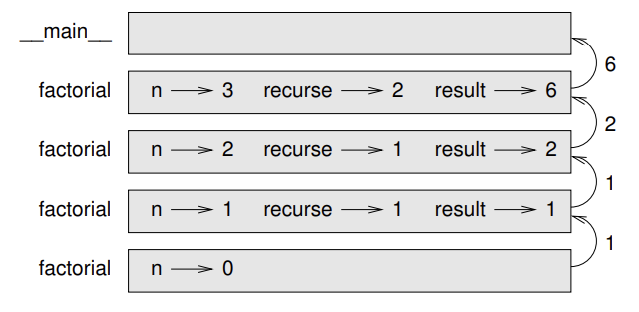
\includegraphics[width=0.5\textwidth]{./images/chapter_6_1.png}
        \caption{Diagrama de Pila.}
        \label{fig:6_1}
        \end{figure}
\section{Salto de fe}

Seguir el flujo de ejecución es una forma de leer programas, pero rápidamente puede volverse abrumador. Una alternativa es lo que yo llamo el "salto de fe". Cuando llegas a una llamada a función, en lugar de seguir el flujo de ejecución, asumes que la función funciona correctamente y devuelve el resultado correcto.

De hecho, ya estás practicando este salto de fe cuando usas funciones incorporadas. Cuando llamas a \texttt{math.cos} o \texttt{math.exp}, no examinas los cuerpos de esas funciones. Simplemente asumes que funcionan porque las personas que escribieron las funciones incorporadas eran buenos programadores.

Lo mismo ocurre cuando llamas a una de tus propias funciones. Por ejemplo, en la Sección 6.4, escribimos una función llamada \texttt{is\_divisible} que determina si un número es divisible por otro. Una vez que nos hemos convencido de que esta función es correcta (examinando el código y probándolo), podemos usar la función sin mirar el cuerpo nuevamente.

Lo mismo ocurre con los programas recursivos. Cuando llegas a la llamada recursiva, en lugar de seguir el flujo de ejecución, deberías asumir que la llamada recursiva funciona (devuelve el resultado correcto) y luego preguntarte: "Asumiendo que puedo encontrar el factorial de $n-1$, ¿puedo calcular el factorial de $n$?" Está claro que puedes, multiplicando por $n$.

Por supuesto, es un poco extraño asumir que la función funciona correctamente cuando no has terminado de escribirla, ¡pero por eso se llama salto de fe!

\section{Un ejemplo más}

Después de \texttt{factorial}, el ejemplo más común de una función matemática definida recursivamente es \texttt{fibonacci}, que tiene la siguiente definición (ver \url{http://en.wikipedia.org/wiki/Fibonacci_number}):

\[
\text{fibonacci}(0) = 0
\]
\[
\text{fibonacci}(1) = 1
\]
\[
\text{fibonacci}(n) = \text{fibonacci}(n-1) + \text{fibonacci}(n-2)
\]

Traducido a Python, se ve así:

\begin{lstlisting}[language=Python]
def fibonacci(n):
    if n == 0:
        return 0
    elif n == 1:
        return 1
    else:
        return fibonacci(n-1) + fibonacci(n-2)
\end{lstlisting}

Si intentas seguir el flujo de ejecución aquí, incluso para valores bastante pequeños de $n$, tu cabeza explotará. Pero según el salto de fe, si asumes que las dos llamadas recursivas funcionan correctamente, entonces está claro que obtienes el resultado correcto sumándolas.

\section{Verificación de tipos}

¿Qué sucede si llamamos a \texttt{factorial} y le damos 1.5 como argumento?

\begin{lstlisting}[language=Python]
>>> factorial(1.5)
RuntimeError: Maximum recursion depth exceeded
\end{lstlisting}

Parece una recursión infinita. ¿Cómo puede ser? La función tiene un caso base: cuando \texttt{n == 0}. Pero si \texttt{n} no es un entero, podemos perder el caso base y recurrir para siempre.

En la primera llamada recursiva, el valor de \texttt{n} es 0.5. En la siguiente, es -0.5. A partir de ahí, se vuelve más pequeño (más negativo), pero nunca será 0.

Tenemos dos opciones. Podemos intentar generalizar la función \texttt{factorial} para que funcione con números de punto flotante, o podemos hacer que \texttt{factorial} verifique el tipo de su argumento. La primera opción se llama función gamma y está un poco más allá del alcance de este libro. Así que optaremos por la segunda.

Podemos usar la función incorporada \texttt{isinstance} para verificar el tipo del argumento. Mientras estamos en eso, también podemos asegurarnos de que el argumento sea positivo:

\begin{lstlisting}[language=Python]
def factorial(n):
    if not isinstance(n, int):
        print('Factorial is only defined for integers.')
        return None
    elif n < 0:
        print('Factorial is not defined for negative integers.')
        return None
    elif n == 0:
        return 1
    else:
        return n * factorial(n-1)
\end{lstlisting}

El primer caso base maneja no enteros; el segundo maneja enteros negativos. En ambos casos, el programa imprime un mensaje de error y devuelve \texttt{None} para indicar que algo salió mal:

\begin{lstlisting}[language=Python]
>>> print(factorial('fred'))
Factorial is only defined for integers.
None
>>> print(factorial(-2))
Factorial is not defined for negative integers.
None
\end{lstlisting}

Si pasamos ambas verificaciones, sabemos que \texttt{n} es un entero no negativo, por lo que podemos probar que la recursión termina.

Este programa demuestra un patrón a veces llamado \textbf{guardián}. Los dos primeros condicionales actúan como guardianes, protegiendo el código que sigue de valores que podrían causar un error. Los guardianes hacen posible probar la corrección del código.

En la Sección 11.4 veremos una alternativa más flexible a imprimir un mensaje de error: generar una excepción.

\section{Depuración}

Dividir un programa grande en funciones más pequeñas crea puntos de control naturales para la depuración. Si una función no funciona, hay tres posibilidades a considerar:

\begin{itemize}
    \item Hay algo mal con los argumentos que recibe la función; se viola una precondición.
    \item Hay algo mal con la función; se viola una postcondición.
    \item Hay algo mal con el valor de retorno o la forma en que se está utilizando.
\end{itemize}

Para descartar la primera posibilidad, puedes agregar una sentencia \texttt{print} al principio de la función y mostrar los valores de los parámetros (y tal vez sus tipos). O puedes escribir código que verifique las precondiciones explícitamente.

Si los parámetros parecen buenos, agrega una sentencia \texttt{print} antes de cada sentencia \texttt{return} y muestra el valor de retorno. Si es posible, verifica el resultado manualmente. Considera llamar a la función con valores que faciliten la verificación del resultado (como en la Sección 6.2).

Si la función parece estar funcionando, mira la llamada a función para asegurarte de que el valor de retorno se esté usando correctamente (¡o que se esté usando!).

Agregar sentencias \texttt{print} al principio y al final de una función puede ayudar a hacer más visible el flujo de ejecución. Por ejemplo, aquí hay una versión de \texttt{factorial} con sentencias \texttt{print}:

\begin{lstlisting}[language=Python]
def factorial(n):
    space = ' ' * (4 * n)
    print(space, 'factorial', n)
    if n == 0:
        print(space, 'returning 1')
        return 1
    else:
        recurse = factorial(n-1)
        result = n * recurse
        print(space, 'returning', result)
        return result
\end{lstlisting}

\texttt{space} es una cadena de caracteres de espacio que controla la sangría de la salida. Aquí está el resultado de \texttt{factorial(4)}:

\begin{lstlisting}[language=Python]
factorial 4
    factorial 3
        factorial 2
            factorial 1
                factorial 0
                returning 1
            returning 1
        returning 2
    returning 6
returning 24
\end{lstlisting}

Si estás confundido acerca del flujo de ejecución, este tipo de salida puede ser útil. Se necesita algo de tiempo para desarrollar andamiaje efectivo, pero un poco de andamiaje puede ahorrar mucha depuración.

\section{Glosario}

\begin{description}
    \item[variable temporal:] Una variable utilizada para almacenar un valor intermedio en un cálculo complejo.
    \item[código muerto:] Parte de un programa que nunca se ejecuta, a menudo porque aparece después de una sentencia \texttt{return}.
    \item[desarrollo incremental:] Un plan de desarrollo de programas destinado a evitar la depuración agregando y probando solo una pequeña cantidad de código a la vez.
    \item[andamiaje:] Código que se usa durante el desarrollo del programa pero que no es parte de la versión final.
    \item[guardián:] Un patrón de programación que usa una sentencia condicional para verificar y manejar circunstancias que podrían causar un error.
\end{description}

\section{Ejercicios}

\textbf{Ejercicio 6.1.} Dibuja un diagrama de pila para el siguiente programa. ¿Qué imprime el programa?

\begin{lstlisting}[language=Python]
def b(z):
    prod = a(z, z)
    print(z, prod)
    return prod

def a(x, y):
    x = x + 1
    return x * y

def c(x, y, z):
    total = x + y + z
    square = b(total)**2
    return square

x = 1
y = x + 1
print(c(x, y+3, x+y))
\end{lstlisting}

\textbf{Ejercicio 6.2.} La función de Ackermann, $A(m, n)$, se define:

\[
A(m, n) =\begin{cases}n+1&\text{si }m=0\\A(m-1,1)&\text{si }m>0\text{ y }n=0\\A(m-1,A(m,n-1))&\text{si }m>0\text{ y }n>0.\end{cases}
\]

Ver \url{http://en.wikipedia.org/wiki/Ackermann_function}. Escribe una función llamada \texttt{ack} que evalúe la función de Ackermann. Usa tu función para evaluar \texttt{ack(3, 4)}, que debería ser 125. ¿Qué sucede para valores mayores de \texttt{m} y \texttt{n}? Solución: \url{https://thinkpython.com/code/ackermann.py}.

\textbf{Ejercicio 6.3.} Un palíndromo es una palabra que se escribe igual al derecho y al revés, como "noon" y "redivider". Recursivamente, una palabra es un palíndromo si la primera y la última letra son iguales y el medio es un palíndromo.

Las siguientes son funciones que toman un argumento de cadena y devuelven la primera, la última y las letras del medio:

\begin{lstlisting}[language=Python]
def first(word):
    return word[0]

def last(word):
    return word[-1]

def middle(word):
    return word[1:-1]
\end{lstlisting}

Veremos cómo funcionan en el Capítulo 8.

\begin{enumerate}
    \item Escribe estas funciones en un archivo llamado \texttt{palindrome.py} y pruébalas. ¿Qué sucede si llamas a \texttt{middle} con una cadena de dos letras? ¿Una letra? ¿Qué pasa con la cadena vacía, que se escribe \texttt{''} y no contiene letras?
    \item Escribe una función llamada \texttt{is\_palindrome} que tome un argumento de cadena y devuelva \texttt{True} si es un palíndromo y \texttt{False} en caso contrario. Recuerda que puedes usar la función incorporada \texttt{len} para verificar la longitud de una cadena.
\end{enumerate}

Solución: \url{https://thinkpython.com/code/palindrome_soln.py}.

\textbf{Ejercicio 6.4.} Un número, \texttt{a}, es una potencia de \texttt{b} si es divisible por \texttt{b} y \texttt{a/b} es una potencia de \texttt{b}. Escribe una función llamada \texttt{is\_power} que tome los parámetros \texttt{a} y \texttt{b} y devuelva \texttt{True} si \texttt{a} es una potencia de \texttt{b}. Nota: tendrás que pensar en el caso base.

\textbf{Ejercicio 6.5.} El máximo común divisor (MCD) de \texttt{a} y \texttt{b} es el número más grande que divide a ambos sin dejar resto.

Una forma de encontrar el MCD de dos números se basa en la observación de que si \texttt{r} es el resto cuando \texttt{a} se divide por \texttt{b}, entonces $\text{mcd}(a,b) = \text{mcd}(b,r)$. Como caso base, podemos usar $\text{mcd}(a,0) = a$.

Escribe una función llamada \texttt{gcd} que tome los parámetros \texttt{a} y \texttt{b} y devuelva su máximo común divisor.

Crédito: Este ejercicio está basado en un ejemplo de \textit{Structure and Interpretation of Computer Programs} de Abelson y Sussman.